%%% The main file. It contains definitions of basic parameters and includes all other parts.

%% Settings for single-side (simplex) printing
% Margins: left 40mm, right 25mm, top and bottom 25mm
% (but beware, LaTeX adds 1in implicitly)
\documentclass[12pt,a4paper]{report}
\setlength\textwidth{145mm}
\setlength\textheight{247mm}
\setlength\oddsidemargin{15mm}
\setlength\evensidemargin{15mm}
\setlength\topmargin{0mm}
\setlength\headsep{0mm}
\setlength\headheight{0mm}
% \openright makes the following text appear on a right-hand page
\let\openright=\clearpage

%% Settings for two-sided (duplex) printing
% \documentclass[12pt,a4paper,twoside,openright]{report}
% \setlength\textwidth{145mm}
% \setlength\textheight{247mm}
% \setlength\oddsidemargin{14.2mm}
% \setlength\evensidemargin{0mm}
% \setlength\topmargin{0mm}
% \setlength\headsep{0mm}
% \setlength\headheight{0mm}
% \let\openright=\cleardoublepage

%% Generate PDF/A-2u
\usepackage[a-2u]{pdfx}

%% Character encoding: usually latin2, cp1250 or utf8:
\usepackage[utf8]{inputenc}

%% Prefer Latin Modern fonts
\usepackage{lmodern}

%% Further useful packages (included in most LaTeX distributions)
\usepackage{amsmath}        % extensions for typesetting of math
\usepackage{amsfonts}       % math fonts
\usepackage{amsthm}         % theorems, definitions, etc.
\usepackage{bbding}         % various symbols (squares, asterisks, scissors, ...)
\usepackage{bm}             % boldface symbols (\bm)
\usepackage{graphicx}       % embedding of pictures
\usepackage{fancyvrb}       % improved verbatim environment
\usepackage{natbib}         % citation style AUTHOR (YEAR), or AUTHOR [NUMBER]
\usepackage[nottoc]{tocbibind} % makes sure that bibliography and the lists
			    % of figures/tables are included in the table
			    % of contents
\usepackage{dcolumn}        % improved alignment of table columns
\usepackage{booktabs}       % improved horizontal lines in tables
\usepackage{paralist}       % improved enumerate and itemize
\usepackage{xcolor}         % typesetting in color

%%% Basic information on the thesis

% Thesis title in English (exactly as in the formal assignment)
\def\ThesisTitle{Thesis title}

% Author of the thesis
\def\ThesisAuthor{Name Surname}

% Year when the thesis is submitted
\def\YearSubmitted{YEAR}

% Name of the department or institute, where the work was officially assigned
% (according to the Organizational Structure of MFF UK in English,
% or a full name of a department outside MFF)
\def\Department{Name of the department}

% Is it a department (katedra), or an institute (ústav)?
\def\DeptType{Department}

% Thesis supervisor: name, surname and titles
\def\Supervisor{Supervisor's Name}

% Supervisor's department (again according to Organizational structure of MFF)
\def\SupervisorsDepartment{department}

% Study programme and specialization
\def\StudyProgramme{study programme}
\def\StudyBranch{study branch}

% An optional dedication: you can thank whomever you wish (your supervisor,
% consultant, a person who lent the software, etc.)
\def\Dedication{%
Dedication.
}

% Abstract (recommended length around 80-200 words; this is not a copy of your thesis assignment!)
\def\Abstract{%
Abstract.
}

% 3 to 5 keywords (recommended), each enclosed in curly braces
\def\Keywords{%
{key} {words}
}

%% The hyperref package for clickable links in PDF and also for storing
%% metadata to PDF (including the table of contents).
%% Most settings are pre-set by the pdfx package.
\hypersetup{unicode}
\hypersetup{breaklinks=true}

% Definitions of macros (see description inside)
%%% This file contains definitions of various useful macros and environments %%%
%%% Please add more macros here instead of cluttering other files with them. %%%

%%% Minor tweaks of style

% These macros employ a little dirty trick to convince LaTeX to typeset
% chapter headings sanely, without lots of empty space above them.
% Feel free to ignore.
\makeatletter
\def\@makechapterhead#1{
  {\parindent \z@ \raggedright \normalfont
   \Huge\bfseries \thechapter. #1
   \par\nobreak
   \vskip 20\p@
}}
\def\@makeschapterhead#1{
  {\parindent \z@ \raggedright \normalfont
   \Huge\bfseries #1
   \par\nobreak
   \vskip 20\p@
}}
\makeatother

% This macro defines a chapter, which is not numbered, but is included
% in the table of contents.
\def\chapwithtoc#1{
\chapter*{#1}
\addcontentsline{toc}{chapter}{#1}
}

% Draw black "slugs" whenever a line overflows, so that we can spot it easily.
\overfullrule=1mm

%%% Macros for definitions, theorems, claims, examples, ... (requires amsthm package)

\theoremstyle{plain}
\newtheorem{thm}{Theorem}
\newtheorem{lemma}[thm]{Lemma}
\newtheorem{claim}[thm]{Claim}

\theoremstyle{plain}
\newtheorem{defn}{Definition}

\theoremstyle{remark}
\newtheorem*{cor}{Corollary}
\newtheorem*{rem}{Remark}
\newtheorem*{example}{Example}

%%% An environment for proofs

\newenvironment{myproof}{
  \par\medskip\noindent
  \textit{Proof}.
}{
\newline
\rightline{$\qedsymbol$}
}

%%% An environment for typesetting of program code and input/output
%%% of programs. (Requires the fancyvrb package -- fancy verbatim.)

\DefineVerbatimEnvironment{code}{Verbatim}{fontsize=\small, frame=single}

%%% The field of all real and natural numbers
\newcommand{\R}{\mathbb{R}}
\newcommand{\N}{\mathbb{N}}

%%% Useful operators for statistics and probability
\DeclareMathOperator{\pr}{\textsf{P}}
\DeclareMathOperator{\E}{\textsf{E}\,}
\DeclareMathOperator{\var}{\textrm{var}}
\DeclareMathOperator{\sd}{\textrm{sd}}

%%% Transposition of a vector/matrix
\newcommand{\T}[1]{#1^\top}

%%% Various math goodies
\newcommand{\goto}{\rightarrow}
\newcommand{\gotop}{\stackrel{P}{\longrightarrow}}
\newcommand{\maon}[1]{o(n^{#1})}
\newcommand{\abs}[1]{\left|{#1}\right|}
\newcommand{\dint}{\int_0^\tau\!\!\int_0^\tau}
\newcommand{\isqr}[1]{\frac{1}{\sqrt{#1}}}

%%% Various table goodies
\newcommand{\pulrad}[1]{\raisebox{1.5ex}[0pt]{#1}}
\newcommand{\mc}[1]{\multicolumn{1}{c}{#1}}


% Title page and various mandatory informational pages
\begin{document}
%%% Title page of the thesis and other mandatory pages

%%% Title page of the thesis

\pagestyle{empty}
\hypersetup{pageanchor=false}
\begin{center}

\centerline{\mbox{
\includegraphics[width=166mm]{../img/logo-en.pdf}}}

\vspace{-8mm}
\vfill

{\bf\Large BACHELOR THESIS}

\vfill

{\LARGE\ThesisAuthor}

\vspace{15mm}

{\LARGE\bfseries\ThesisTitle}

\vfill

\Department

\vfill

{
\centerline{\vbox{\halign{\hbox to 0.45\hsize{\hfil #}&\hskip 0.5em\parbox[t]{0.45\hsize}{\raggedright #}\cr
Supervisor of the bachelor thesis:&\Supervisor \cr
\noalign{\vspace{2mm}}
Study programme:&\StudyProgramme \cr
\noalign{\vspace{2mm}}
Study branch:&\StudyBranch \cr
}}}}

\vfill

% Zde doplňte rok
Prague \YearSubmitted

\end{center}

\newpage

%%% Here should be a bound sheet included -- a signed copy of the "bachelor
%%% thesis assignment". This assignment is NOT a part of the electronic
%%% version of the thesis. DO NOT SCAN.

%%% A page with a solemn declaration to the bachelor thesis

\openright
\hypersetup{pageanchor=true}
\pagestyle{plain}
\pagenumbering{roman}
\vglue 0pt plus 1fill

\noindent
I declare that I carried out this bachelor thesis independently, and only with the cited
sources, literature and other professional sources. It has not been used to obtain another
or the same degree.

\medskip\noindent
I understand that my work relates to the rights and obligations under the Act No.~121/2000 Sb.,
the Copyright Act, as amended, in particular the fact that the Charles
University has the right to conclude a license agreement on the use of this
work as a school work pursuant to Section 60 subsection 1 of the Copyright~Act.

\vspace{10mm}

\hbox{\hbox to 0.5\hsize{%
In \hbox to 6em{\dotfill} date \hbox to 6em{\dotfill}
\hss}\hbox to 0.5\hsize{\dotfill\quad}}
\smallskip
\hbox{\hbox to 0.5\hsize{}\hbox to 0.5\hsize{\hfil Author's signature\hfil}}

\vspace{20mm}
\newpage

%%% Dedication

\openright

\noindent
\Dedication

\newpage

%%% Mandatory information page of the thesis

\openright

\vbox to 0.5\vsize{
\setlength\parindent{0mm}
\setlength\parskip{5mm}

Title:
\ThesisTitle

Author:
\ThesisAuthor

\DeptType:
\Department

Supervisor:
\Supervisor, \SupervisorsDepartment

Abstract:
\Abstract

Keywords:
\Keywords

\vss}

\newpage

\openright
\pagestyle{plain}
\pagenumbering{arabic}
\setcounter{page}{1}


%%% A page with automatically generated table of contents of the bachelor thesis

\tableofcontents

%%% Each chapter is kept in a separate file
\chapter*{Introduction}
\addcontentsline{toc}{chapter}{Introduction}

\noindent
Anyone with internet access must have noticed the rapid development of artificial intelligence (AI). What used to be science fiction in the past (not that many years ago) is now becoming more and more relevant. Some people are fascinated and others are terrified by the capabilities of modern AI technologies, ranging from large language models (LLM) to generative video makers with precise details.

\medskip\noindent
We can have lengthy and deeply philosophical discussions on the definition and meaning of intelligence. Every living being has some kind of intelligence. Humans, animals, insects, and even trees have some level of intelligence and consciousness. We may not conclude on the final form of this definition, but surely we will all agree that a substantial part of intelligence is decision-making and planning. From the variety of all possible actions, we choose one that is the most suitable and optimal for the current situation. In situations where we want to attain a complex goal, we need to use our intelligence and create a plan, i.e., a sequence of valid actions that will change the current state of the world to the desired one.

\medskip\noindent
This thesis concerns the Hierarchical Task Network (HTN) which is the way most people think about problems and ways of solving them. Having some abstract and high-level tasks, we may decompose these tasks into subtasks that may be later again decomposed or executed right away. A high-level task is accomplished when all of its subtasks are accomplised. HTN can express different planning domains more compactly and intuitively than classical planning, which will be discussed in this thesis as well.

\section*{Motivation}

\noindent
The theory of classical and hierarchical planning is closely related to the theory of Automata~and~Grammars~\cite{complexity}~\cite{langclassification}~\cite{cmyk}. For this reason, we can utilize concepts, knowledge, and well-known structures from the theory of Automata~and~Grammars and apply them to the field of planning. Planning and especially hierarchical planning is widely used in AI and other similar fields of informatics.

\medskip\noindent
If we want to improve AI, then we need to improve planning, which is part of the concept of intelligence, as we discussed earlier. If we want to improve some theoretical knowledge, then we need to do theoretical research in that field. Hence, this bachelor's thesis was created, to at least somehow help the international community of researchers in this particular field. The impact will be most likely close to none, but it is important to remember the saying, "Rome was not built in a day".

\section*{Goal}

\noindent
\xxx{TODO}

\section*{Structure}

\noindent
In chapters one and two, we will describe and define classical planning and HTN planning, respectively. There are many different ways of representing both planning models, however, we will outline only the most known representations. In the third chapter, we will characterize various semantics of HTN planning. That is, what is the meaning of HTN models, and how we should think about them. Finally, the fourth chapter shows some transformations, that might help achieve prerequisites for particular HTN planners, for example, to compile away unsupported features.
\chapter{Classical {P}lanning}

\medskip\noindent
Before we dive into HTN planning, it's essential to understand its predecessor, which is classical planning or, as it is called in some literature, STRIPS planning~\cite{strips}. Classical planning is lightweight in the sense that it is easier to get into the theory of planning (independently on a representation of planning, which will be discussed in this chapter) and it is easier to describe domains of problems. The concept of classical planning is similar to the theory of Automata and Grammars (deterministic finite automaton (DFA), to be precise). There are different states of the world as well as actions that change one state to another. An action in classical planning can be viewed as a state transition function $\gamma: S \times A \rightarrow S$, where $S$ and $A$ denote the sets of all states and actions, respectively. If an action is applicable to a state then there will be a state transition, otherwise it will be undefined. The set of goal states, $S_g \subseteq S$, is analogous to a set of accepting states. The planning problem then can be reduced to a problem of searching paths in a directed graph.

\medskip\noindent
Although this approach of classical planning is simple and straightforward, it has one crucial flaw which makes it unusable in practice. Imagine a planning domain that describes a warehouse. If we have five locations, three piles of containers per location, three robots, and one hundred containers, then there are $10^{277}$ states~\cite{nau}, which is much more than the number of atoms in the observable universe. And that is just a simple small domain with a small amount of objects. For this purpose, we need to use better ways of representing classical planning, which will be called \emph{state-transition system}. We will briefly describe two possible representations: \emph{set-theoretic representation} and \emph{classical representation}.

\medskip\noindent
In both representations, the idea is to use more compact ways of defining a state of the world and actions that change the state. Instead of having a set of all states $S$, we will have a finite set of proposition symbols $P = \{p_1,\dots,p_n\}$ in \emph{set-theoretic representation} and a first-order language $\mathcal{L}$ in \emph{classical representation}. Both, $P$ and $\mathcal{L}$ describe properties and features of the world. Each state is then defined by a set of properties, which are true in that state and every other property is false. This feature is called closed world assumption. Both of these representations have the same expressive power~\cite{nau}. 

\medskip\noindent
All of the following definitions are correspondent and equivalent to the definitions in the book \emph{Automated Planning: theory and practice (Chapter 2)}~\cite{nau}.

\section{Set-Theoretic Representation}

\begin{defn}\label{def01:1}
  Let $P = \{p_1,\dots,p_n\}$ be a finite set of propositional symbols, which will model properties of a world. Then $\Sigma = (S, A, \gamma)$ is a \emph{planning domain} on $P$. $S$, $A$, and $\gamma$ denote the set of all states, set of all actions, and the \emph{state-transition function}, respectively, such that:

  \begin{itemize}
      \item $S \subseteq 2^{P}$, each state $s \in S$ holds in properties of the world, that are true. Other propositional symbols $p \in P$, $p \notin s$ do not hold in a state $s$.
      
      \item Each action $a \in A$ is defined as a triple of sets describing the preconditions and changes to a current state. Action $a \in A$ will be denoted as \mbox{$a=(pre(a), \text{eff}^{\,\,-}(a), \text{eff}^{\,\,+}(a)) \in  2^{P} \times 2^{P} \times 2^{P}$}, where $pre(a)$ stands for preconditions that must be true in a state to apply this action, meanwhile $\text{eff}^{\,\,-}(a)$ and $\text{eff}^{\,\,+}(a)$ describe changes to the state or, in other words, negative and positive effects\footnote{In some literature these sets are called: add list, delete list.}. We require $\text{eff}^{\,\,-}(a) \cap \text{eff}^{\,\,+}(a) = \emptyset$ for every $a \in A$, because otherwise it does not make any sense. Having a state $s \in S$, an action $a \in A$ is \emph{applicable} to state $s$, if and only if $pre(a) \subseteq s$ (it might be convenient to specify $pre^{-}(a)$ and $pre^{+}(a)$ to denote positive and negative preconditions).
      
      \item Having $s \in S$ and an action $a \in A$ that is \emph{applicable} to state $s$, \emph{state-transition} function $\gamma$ is defined as follows: $\gamma(s,a)=(s-\text{eff}^{\,\,-}(a)) \cup \text{eff}^{\,\,+}(a)$, otherwise it is undefined.
      \item $S$ must have a property that for every $s \in S$ and $a \in A$ that is \emph{applicable} to $s$, $\gamma(s,a) \in S$. This way we do not have to know all of the states in advance. All we need is a set of actions $A$ and some initial state $s_0 \in S$, then we can find all reachable states using Breadth-First Search (BFS), Depth-First Search (DFS), or some other searching algorithms.
  \end{itemize}
\end{defn}

\begin{defn}\label{def01:2}
  A \emph{planning problem} is a triple $\mathcal{P}=(\Sigma,s_o,g)$, such that:

  \begin{itemize}
    \item $\Sigma = (S, A, \gamma)$ is a \emph{planning domain} on $P$.
    
    \item $s_0 \in S$ is an \emph{initial state}.
    
    \item $g \subseteq P$ is a set of \emph{goal proposition symbol}, which must be true in the state after the final action of a plan. $S_g=\{s \in S | g \subseteq s\}$ is a set of goal states, i.e., states that satisfy the \emph{planning problem}~$\mathcal{P}.$
  \end{itemize}
\end{defn}

\noindent
Because the set of \emph{propositional symbol} $P$ is finite, sets of states, actions, and state-transition function are also finite.

\begin{defn}\label{def01:3}
  A \emph{plan} in a \emph{planning domain} $\Sigma$ is a finite sequence of actions $\pi=(a_1,\dots,a_k)$, where $k \geq 0$ and $(\forall a \in \pi) a \in A$. The \emph{plan} $\pi$ is \emph{applicable} to a state $s_0 \in S$, if and only if a sequence of states $(s_0,\dots,s_k)$ exist, such that: \mbox{$(1 \leq i \leq k)$} $s_{i-1} \subseteq pre(a_i)$ and $s_i = \gamma(s_{i-1},a_i) = ((s_{i-1}-\text{eff}^{\,\,-}(a_i)) \cup \text{eff}^{\,\,+}(a_i))$ is defined. Otherwise, the \emph{plan} $\pi$ is invalid. 

  \medskip\noindent
  In other words, a \emph{plan} $\pi=(a_1,\dots,a_k)$ is \emph{applicable} to a state $s_0$, if and only if a \emph{plan} $\pi'=(a_2,\dots,a_k)$ is \emph{applicable} to a state $s_1=\gamma(s_0,a_1) \in S$.

  \medskip\noindent
  Having a \emph{plan} $\pi=(a_1,\dots,a_k)$ and a state $s \in S$, we will abuse the notation to let $\gamma(s,\pi)$ denote a state $s_k \in S$, where we get after applying the sequence of actions of a plan, i.e.,
    \[
    \gamma(s,(a_1,\dots,a_k))=
    \begin{cases}
    s, & \text{if $k=0$ (there are no actions)},\\
    \gamma(\gamma(s,a_1),(a_2,\dots,a_k)), & \text{if k $>$ 0, $a_1$ is \emph{applicable} to $s$}, \\
    undefined, & \text{otherwise}.
    \end{cases}
    \]
\end{defn}



\begin{defn}\label{def01:4}
    A \emph{solution} to a \emph{planning problem} $\mathcal{P}=(\Sigma,s_o,g)$ is a plan $\pi=(a_1,\dots,a_k)$ that is \emph{applicable} to $s_0$, which changes the initial state $s_0$ to a state that satisfies \emph{goal propositional symbols}: $\gamma(s_0,\pi)$ is defined and $g \subseteq \gamma(s_0,\pi)$ (equivalent to $\gamma(s_0,\pi) \in S_g$).
\end{defn}

\noindent
For a \emph{planning problem} there might be many \emph{solutions}, moreover, there might be an infinite number of \emph{solutions} if there are states that can be visited repeatedly, (e.g. we might have two adjacent locations in a domain, that can be visited cyclically without any constraints).

\medbreak\noindent
It is easy to see that for each \emph{planning problem} $\mathcal{P}$ with nonempty set of \emph{solutions} (there exist a \emph{plan} $\pi$ such that $\pi$ is a solution to a $\mathcal{P}$) there exist at least one \emph{minimal solution} $\pi=(a_1,\dots,a_k)$, i.e., there is no \emph{solution} $\pi'=(a_1,\dots,a_j)$ such that $j < k$. There might be many different \emph{minimal solutions} but all of them share the same length.


\begin{example}\label{ex01:1}
    \begin{figure}
        \centering
        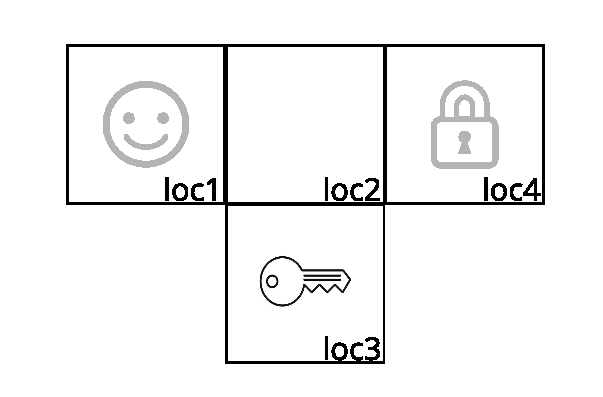
\includegraphics{img/output_mares_key1.pdf}
        \caption{Initial state of a simple planning domain}
        \label{fig01:1}
    \end{figure}
    
    Imagine a simple planning domain (Figure~\ref{fig01:1}) that can represent states in an uncomplicated maze-like game. We have four game locations, a player character, a key, and a locked door (illustrated by a \emph{loc4}). The character can move freely between locations but if he wants to enter \emph{loc4}, then he needs a key that can be picked at the \emph{loc3} (but cannot be discarded later on). Now we will define a planning problem $\mathcal{P}=(\Sigma,s_0,g)$ for this domain $\Sigma=(S,A,\gamma)$ more formally:
    
\end{example}

\begin{itemize}
    \item $P=\{${at-loc1,at-loc2,at-loc3,at-loc4,key-picked}$\}$,
    
    \item $S=\begin{aligned}[t]
    &\{\{ \mathrm{at\text{-}loc1}\}, \{ \mathrm{at\text{-}loc2}\}, \{ \mathrm{at\text{-}loc3}\}, \{ \mathrm{at\text{-}loc1,key\text{-}picked}\},\\
    & \{ \mathrm{at\text{-}loc2,key\text{-}picked}\},
    \{ \mathrm{at\text{-}loc3,key\text{-}picked}\}, \{ \mathrm{at\text{-}loc4,key\text{-}picked}\}\},
    \end{aligned}$

    \item $A=\begin{aligned}[t]
    &\mathrm{\{move12,move21,move23,move32,move24,move42,pick\}, where:} \\
    &\mathrm{move12 = (\{at\text{-}loc1\},\{at\text{-}loc1\},\{at\text{-}loc2\});} \\
    &\mathrm{move21 = (\{at\text{-}loc2\},\{at\text{-}loc2\},\{at\text{-}loc1\});} \\
    &\mathrm{move23 = (\{at\text{-}loc2\},\{at\text{-}loc2\},\{at\text{-}loc3\});} \\
    &\mathrm{move32 = (\{at\text{-}loc3\},\{at\text{-}loc3\},\{at\text{-}loc2\});} \\
    &\mathrm{move24 = (\{at\text{-}loc2,key\text{-}picked\},\{at\text{-}loc2\},\{at\text{-}loc4\});} \\
    &\mathrm{move42 = (\{at\text{-}loc4\},\{at\text{-}loc4\},\{at\text{-}loc2\});} \\
    &\mathrm{pick = (\{at\text{-}loc3\},\{\},\{key\text{-}picked\}),}
    \end{aligned}$ 

    \item $\gamma$ as defined in Definition~\ref{def01:1},

    \item $s_0 = \{ \mathrm{at\text{-}loc1}\}$ (Figure~\ref{fig01:1}),

    \item $g = \{ \mathrm{at\text{-}loc4, key\text{-}picked}\}$.
\end{itemize}

\noindent
Example~\ref{ex01:1} shows us a complete description of a \emph{planning domain} $\Sigma$ and a \emph{planning problem} $\mathcal{P}$. There is one and only \emph{minimal solution} which is $\pi=(\mathrm{move12,move23,pick,move32,move24})$. On the other hand, there is an infinite amount of \emph{solutions}. We might go to the loc3 and apply the action pick as many times as we desire, thus generating an infinite amount of \emph{solutions}.

\medskip\noindent
With knowledge of the particular domain, we can adjust the domain without losing any domain's specifics. For example, we might alter the set of the \emph{goal proposition symbols} $g$ to be $g=\mathrm{\{at\text{-}loc4\}}$ because we know that it is impossible to enter loc4 without having a key picked up at the loc3.

\medskip\noindent
The set of states $S$ contains all reachable states from the initial state $s_0$, other unreachable states might be added to the $S$ but they are not needed. For example, the state \{at-loc1,at-loc2\} is contradictory because we cannot be at two locations simultaneously. Likewise states \{\}, \{key-picked\}, \{at-loc4\} are also meaningless.

\medskip\noindent
The concept of the key in this domain is depicted as a \emph{propositional symbol} key-picked. This simplification does not take into account the location of a key because it is not needed in this domain. Once the key is picked, it will be implicitly located at the same location as the character. Hence, the action pick is \emph{applicable} more than once in a \emph{plan}.

\begin{figure}
    \centering
    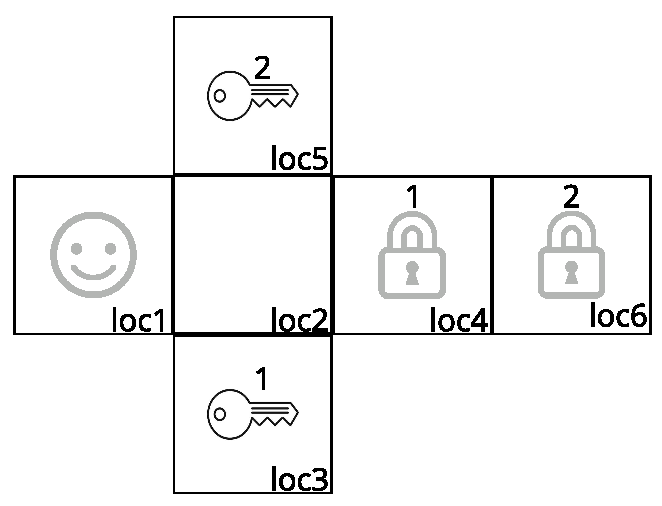
\includegraphics{img/output_mares_key2.pdf}
    \caption{Extended planning domain of a maze-like game}
    \label{fig01:2}
\end{figure}

\begin{example}\label{ex01:2}
    Let's consider an extension of this domain by adding two new locations, and another key (Figure~\ref{fig01:2}). Only this time we want to model a new constraint that allows at most one key to be held at a time. There are numerous ways of modeling this planning domain. For instance, we might introduce new \emph{propositional symbols}: \emph{key1-picked, key2-picked, door1-opened, door2-opened}. If we wanted to model the locations of keys, we would need to include many new \emph{propositional symbols} of the form \emph{key1-at-loc1, key1-at-loc2}, and so on. Also, we would need new \emph{actions} that would consider the locations of a key and the character. New actions may look like this: \emph{pick-key1-at1 = (\{at-loc1,key1-at-loc1\},\{key2-picked\},\{key1-picked\}), move12-with-key1 = (\{at-loc1,key1-at-loc1\},\{at-loc1,key1-at-loc1\},\{at-loc2,key1-at-loc2\})} and so on. This enumeration of possible substates might result in an enormous set of \emph{propositional symbols} and other related sets \emph{\cite{nau}~{(2.2.4 Properties of the Set-Theoretic Representation)}}. An elaborate solution that fixes this problem is discussed in the following chapter.
\end{example}

\section{Classical Representation}\label{class_repre}

\noindent
\emph{Classical representation} of planning improves \emph{set-theoretic representation} by introducing a first-order language $\mathcal{L}$ that consists of a finite number of constant symbols (similar to a set of \emph{propositional symbols} defined in Definition~\ref{def01:1}), predicate symbols, and other symbols for the representation of \emph{planning operators}. We do not allow any functional symbols in $\mathcal{L}$ because then we would have complications with modeling finite domains. A state in \emph{classical representation} is defined as a set of grounded logical atoms of $\mathcal{L}$.

\begin{example}\label{ex01:3}
    Before we start with definitions, we will look at Figure~\ref{fig01:1} from the perspective of \emph{classical planning}. We want to model the player, key, locations, and locked door. Thus, the set of constant symbols is \emph{\{player,loc1,loc2,loc3,loc4} \emph{,key1,nothing,door\}}. The constant symbol \emph{nothing} represents that the player's inventory is empty. With this knowledge, we can represent the initial state of Figure~\ref{fig01:1} to be $s_0=\{\mathrm{adjacent(loc1,loc2)},\mathrm{adjacent(loc2,loc1)},\mathrm{adjacent(loc2,loc3)}, \\ \mathrm{adjacent(loc3,loc2)}, \mathrm{adjacent(loc2,loc4)},\mathrm{adjacent(loc4,loc2)}, \mathrm{at(player,loc1)}, \\ \mathrm{holds(player,nothing)}, \mathrm{locked(door)}\}$. Some logical atoms will remain the same throughout all possible states, e.g. \emph{adjacent(loc1,loc2)}, meanwhile other atoms like \emph{at(player,loc1)} or \emph{holds(player,nothing)} will change after the application of proper actions.
\end{example}

\medskip\noindent
Now we will define \emph{planning operators} in \emph{classical planning}. \emph{Planning operators} do not contain any constant symbols, only variable symbols. A grounded instance of an operator is an action that can be part of a \emph{plan}.

\pagebreak

\begin{defn}\label{def01:5}
    A \emph{planning operator} is a triple $o = (name(o),precond(o), \\ \text{eff}(o))$, where:

        \begin{itemize}
            \item $name(o)$ is of a form $n(x_1,\dots,x_k)$, where $n$ is a \emph{operator symbol} and must be unique in $\mathcal{L}$ and $x_1,\dots,x_k$ represent variable symbols that appear in an operator,

            \item $precond(o)$ and $\text{eff}(o)$ generalize preconditions and effects of \emph{set-theoretic representation}. These sets contain positive and negative logical literals.
        \end{itemize}

    Let $O$ denote a set of all \emph{planning operators} as specified above.
\end{defn}

\medskip\noindent
In some literature, the usage of $name(o)$ is not specified, rather the multiset of grounded operators (actions) is assumed. The essence of $name(o)$ is in the planning phase. We might have multiple grounded instances of operators that might use the equivalent constant symbols. To help differentiate a \emph{planning operator} from an instance of a \emph{planning operator}, the $name(o)$ might come in handy. $name(o)$ refers unambiguously to one specific \emph{planning operator}. We will omit the usage $name(o)$ because the meaning will be obvious from the context.


\begin{example}\label{ex01:4}
    In this example, we will look at some possible \emph{planning operators} that might be used in Figure~\ref{fig01:2} (we will use new predicate symbols that were not specified yet):

    \begin{itemize}
        \item \emph{move(player,location1,location2)} \\
        precond: \emph{adjacent(location1,location2), at(player,location1), \neg locked(location2)} \\
        effects: \emph{\neg at(player,location1), at(player, location2)}

        \item \emph{pickup-key(player,key,location)} \\
        precond: \emph{at(player,location), at(key,location), holds(player,nothing)} \\
        effects: \emph{\neg holds(player,nothing), \neg at(key,location), holds(player,key)}

        \item \emph{drop-key(player,key,location)} \\
        precond: \emph{at(player,location), holds(player,key)} \\
        effects: \emph{\neg holds(player,key), at(key,location), holds(player,nothing)}

        \item \emph{open-door(player,location1,location2, key)} \\
        precond: \emph{adjacent(location1,location2), locked(location2), at(player,location1), key-opens-door(key,location2), holds(player,key)} \\
        effects: \emph{\neg locked(location2)}
    \end{itemize}
\end{example}

\medskip\noindent
In the Example~\ref{ex01:4} predicate symbols adjacent(l1,l2) and key-opens-door(key,location) are describing static properties of a domain that will never change and thus, will never appear in effects of \emph{planning operators}. On the other hand, predicate symbols like at(player/key,location), locked(location), or holds(player, key) will change and therefore will occur in effects of \emph{planning operators}.

\begin{defn}\label{def01:6}
Let us be given a state $s \in S$ and an action (ground instance of a \emph{planning operator}) $a$. If $precond^{+}(a) \subseteq s$ and $precond^{-}(a) \cap s = \emptyset$, where $precond^{+}(a)$ denotes a set of all positive atoms in $precond(a)$ and $precond^{-}(a)$ denotes a set of all atoms whose negation is in $precond(a)$, then $a$ is \emph{applicable} to $s$ and $\gamma(s,a)=(s-\text{eff}^{\,\,-}(a)) \cup \text{eff}^{\,\,+}(a)$. $\text{eff}^{\,\,-}(a)$ and $\text{eff}^{\,\,+}(a)$ are analogous to $precond^{-}(a)$ and $precond^{+}(a)$, respectively.
\end{defn}

\begin{defn}\label{def01:7}
Having a first-order language $\mathcal{L}$ with a finite amount of constant and predicate symbols and no functional symbols, the \emph{classical planning domain} in $\mathcal{L}$ is a state-transition system $\Sigma = (S,A,\gamma)$ such that:

    \begin{itemize}
        \item $S \subseteq 2^{\displaystyle \{all~ground~atoms~of~\mathcal{L}\}}$,
        
        \item $A =~$\{all ground instances of operators in $O$\},
        
        \item $\gamma$ is analogous Definition~\ref{def01:1},
        
        \item $S$ is closed under $\gamma$ in the same manner as in Definition~\ref{def01:1}.
    \end{itemize}
\end{defn}

\begin{defn}\label{def01:8}
A \emph{classical planning problem} is corresponding to \emph{set-theoretic planning problem}, it is defined as $\mathcal{P} = (\Sigma,s_0,g)$, where:

    \begin{itemize}
        \item $\Sigma = (S,A,\gamma)$ is a \emph{classical planning domain},
        
        \item $s_0 \in S$ is an initial state
        
        \item $g$ is a set of literals.
    \end{itemize}
\end{defn}

\chapter{Hierarchical {P}lanning}

\medskip\noindent
Now that we have understood classical planning, we can move on to hierarchical planning or Hierarchical Task Network (HTN), to be precise. In HTN the goal alone is not to find an \emph{applicable plan} that will meet all of the criteria of the \emph{planning problem}. HTN focuses on accomplishing some set of tasks by decomposing them into sub-tasks with constraints like ordering and state conditions. A task is accomplished immediately upon all of his sub-tasks are accomplished. HTN is an extension of classical planning which gives us clues on how to find the proper \emph{plan}.

\medskip\noindent
As in classical planning, there are states of the world represented by the set of \emph{proposition symbols} or \emph{logical atoms} that are true in a state. We can \emph{apply actions} to states if the preconditions of \emph{actions} are satisfied (held in a state). These \emph{actions} will be called \emph{primitive tasks} in HTN. These tasks are executable right away and they change the current state to another one by applying negative and positive effects. In addition to \emph{primitive tasks} there are \emph{non-primitive tasks}. We will call them \emph{compound tasks}. These tasks cannot be executed and \emph{applied to a state}, rather they have to be decomposed into a set of sub-tasks using decomposition \emph{methods}, both \emph{primitive} and \emph{compound}. Having an \emph{initial task network}, that is a set of tasks and a set of constraints, the goal is to decompose all tasks into \emph{primitive tasks} and find an ordering of these tasks so that the constraints are not violated. After doing so, it is important to check that the resulting \emph{plan} (a sequence of \emph{primitive tasks}) is a valid \emph{plan} and can be \emph{applied} to an \emph{initial state}.

\medskip\noindent
All of the following definitions are correspondent and equivalent to the definitions in the book \emph{Automated Planning: theory and practice (Chapter 11)}~\cite{nau} and other publications~\cite{langclassification}~\cite{cmyk}~\cite{ondrckova2023semantics}~\cite{ondrckova2024empty}.

\section{HTN Planning}

\begin{defn}\label{def02:9}
    A \emph{task network} is a pair $\omega = (U,C)$, where $U$ is a set of \emph{tasks} (primitive and compound) and $C$ is a set of constraints.
    
    For a \emph{solution} (\emph{plan}) to be valid we need to satisfy all of the constraints listed in $C$. We identify four types of constraints:

    \begin{itemize}
        \item $t_i \prec t_j$ where $t_i,t_j \in U$: an \emph{ordering-constraint} meaning that in every valid \emph{solution} the last \emph{primitive task} (\emph{action}) in the \emph{solution} to which $t_i$ decomposes must precede the first \emph{primitive task} (\emph{action}) in the \emph{solution} to which $t_j$ decomposes,
        
        \item $before(l,U')$: \emph{before-constraint} symbolizing that in every valid \emph{solution} the literal $l$ must hold in a state right before the \emph{application} of a first \emph{action} to which $U' \subseteq U$ decomposes,
    
        \item $after(U',l)$: \emph{after-constraint} is similar to \emph{before-constraint} with the difference that the literal $l$ must hold in a state right after the last \emph{action} to which set $U'$ decomposes,
    
        \item $between(U',l,U'')$: \emph{between-constraint} is saying that the literal $l$ must hold in all states starting after the last \emph{action} of $U'$ and lasting until the state right before the \emph{application} of a first \emph{action} of $U''$.
    \end{itemize}

    We will say that the \emph{task network} is \emph{primitive} if and only if, all of the tasks are \emph{primitive}. A \emph{task network} having at least one \emph{compound task} will be called \emph{non-primitive}.
\end{defn}

\medskip\noindent
The most used \emph{state-constraint} is \emph{a before-constraint} which can be modeled in various HTN planners. The usage and application of this constraint is obvious. Before the beginning of a task, we want to hold some preconditions that are significant for that particular task. For example, a user needs to input all of the information before he can continue with the paying; a player needs to complete all of the quests before he can move on to the next stage, or a warehouse robot needs to have permission set before he can execute some real-life tasks. Analogous \emph{after-constraint} has different use cases. We might use this constraint on the last task in \emph{the task network} to signalize our intentions which are not modeled with the tasks themselves. For example, we want to deallocate resources of the process after the completion, or we want to give a player new abilities after the completion of many tasks that might interleave. This constraint can be used as a shortcut in difficult models where the person responsible for the modeling cannot enumerate and decide the ordering of tasks perfectly. \emph{The between-constraint} represents an interval of states which hold some property. For example, we want a player to have a specific item in his inventory after the completion of one task and lasting until the other tasks, or an autonomous robot must hold a crate in all states meanwhile he moves from one location to another (possibly doing other unrelated things).

\medskip\noindent
In accordance with the Definition~\ref{def01:5}, the more formal definition~\cite{complexity}~\cite{langclassification}~\cite{nau} of the \emph{task network} would contain some function $\alpha: U \rightarrow N$, which would map instances of \emph{primitive} and \emph{compound tasks} to the set of names of all \emph{tasks}. This function would allow us to have multiple instances of the same \emph{task} in the set of tasks $U$, each with a unique identifier. We will omit a function $\alpha$ because its context will always be clear.

\begin{defn}\label{def02:10}
    A \emph{method} is a triple $m = (compound(m),subtasks(m), \\ constraints(m))$, where $compound(m)$ is a \emph{compound  task} and $(subtasks(m), \\ constraints(m))$ is a \emph{task network}. $constraints(m)$ operate only with the tasks in $subtasks(m)$. Having a \emph{task network} $\omega=(U,C)$, \emph{compound task} $c \in U$, and an instance of \emph{method} $m$ from $M$. Then $m$ decomposes $c$ into $subtasks(m)$, creating a new \emph{task network} $\omega'=(U',C')$ of a form:

    \[
    \delta(\omega,c,m) = ((U-\{c\}) \cup subtasks(m), C' \cup constraints(m)),
    \]

    \noindent
    where $C'$ is a modification of $C$:

    \begin{itemize}
        \item replace each \emph{ordering-constraint} containing $c$ with new ones containing $subtasks(m)$, i.e., $\forall c' \in subtasks(m): c \prec x$ is replaced with $c' \prec x$ and $x \prec c$ is replaced with $x \prec c'$,
        
        \item replace each \emph{before-, after-, between-constraint} containing $c$ with new ones containing $subtasks(m)$. For example, we would replace \emph{before-constraint} $before(l,V)$ with $before(l,(V - \{c\}) \cup subtasks(m))$.
    \end{itemize}
\end{defn}

\medbreak\noindent
It is highly convenient to write planning \emph{methods} as rewriting rules~\cite{ondrckova2023semantics}:

\[
T \rightarrow T_1,\dots,T_k \quad [C].
\]

\noindent
This rewriting rule symbolizing a \emph{method} is saying as follows: A \emph{method} which decomposes the \emph{compound task} $T$ into sub-tasks $T_1,\dots,T_k$ under the constraints $C$.

\medbreak\noindent
Definition~\ref{def02:10} works well for \emph{planning domains} without \emph{empty methods} (a \emph{method} that decomposes compound task into the empty set of subtasks). Using \emph{an empty method} creates undefined behavior because the decomposed compound task is removed from all constraints and thus it is unclear where the specified constraint should be checked. For this reason, we will later redefine \emph{method} decomposition. 

\begin{defn}\label{def02:11}
    A \emph{(HTN) planning domain} is a quadruple $\mathcal{D} = (\mathcal{L} \ / \ P, O, C, M$), where $\mathcal{L} \ / \ P$ and $O$ are first-order language (\emph{set of propositional symbols}) and a set of \emph{operators}, respectively, as described in the section \nameref{class_repre}, $C$ is a set of \emph{compound tasks} and $M$ represents a set of all \emph{methods}.

    \noindent
    \emph{Planning domain} will be referred to as \emph{totally-ordered} if all of the \emph{methods} in $M$ and the \emph{initial task network} are \emph{totally-ordered} (there is a total strict ordering of sub-tasks). \emph{Planning domains} that are not \emph{totally-ordered} will be referred to as \emph{partially-ordered}.
\end{defn}

\medskip\noindent
A first-order language $\mathcal{L}$ can be easily interchanged for a set of \emph{propositional symbols} $P$ due to the equivalent expressive power of \emph{set-theoretic representation} and \emph{classical representation}~\cite{nau}.

\begin{defn}\label{def02:12}
    A \emph{(hierarchical) planning problem} is a triple $\mathcal{P} = (s_0,\omega,\mathcal{D})$ that consists of \emph{initial state} of the world $s_0$, \emph{initial task network} $\omega$ and a \emph{planning domain} $\mathcal{D}$.
\end{defn}

\begin{defn}\label{def02:13}
    A \emph{solution} to the \emph{planning problem} $\mathcal{P}$ is a \emph{plan} $\pi=(a_1,\dots,a_k)$. This sequence of \emph{actions} is assembled from a \emph{primitive task network} $\omega'=(U', C'), \; U' = 
 \{a_i \; | \; 1 \leq i \leq k\}$, after the application of a sequence of \emph{methods} from $M$ to the \emph{initial task network} $\omega$. A \emph{solution} $\pi$ needs to be valid, i.e., $\gamma(s_0,\pi)$ is not undefined and also needs to satisfy all of the constraints in $C'$. That is:
    
    \begin{itemize}
        \item $a_i \prec a_j \implies i < j$,
        
        \item $before(l, V) \implies l \in s_{min\{i \; | \; a_i \; \in \; V\} \; - \; 1}$ (if the literal $l$ is negative then it must not be in a state, same applies for other constraints),
        
        \item $after(V,l) \implies l \in s_{max\{i \; | \; a_i \; \in \; V\}}$,
        
        \item $between(V',l,V'') \implies (\forall j, \; max\{i \; | \; a_i \; \in \; V'\} \; \leq \; j \; < \; min\{i \; | \; a_i \; \in \; V''\}: l \; \in \; s_j)$.
    \end{itemize}
    
    By $l$ we mean a ground instance of a literal $l$ (in the case of \emph{set-theoretic} representation it would be $p \in P$).
\end{defn}

\section{HTN and Context-free Grammars}

\medskip\noindent
With the knowledge acquired in the previous sections, we can try to map planning definitions and structures to the definitions and structures of the theory of Automata and Grammars. By doing so, we would be able to utilize already discovered knowledge and algorithms. Furthermore, it will allow us to prove different language classifications~\cite{langclassification}.

\medskip\noindent
The simplest example is to map \emph{classical planning problem} to the equivalent DFA, and vice versa. The mapped DFA generates all of the \emph{solutions}, i.e., \emph{plans} that are valid, \emph{applicable} to the \emph{initial state} $s_0$ and satisfy the goal $g$.

\begin{thm}\label{thm02:1}
    For every \emph{classical planning problem $\mathcal{P} = (S, A, \gamma, s_0, g)$}, where $(S, A, \gamma)$ is a \emph{planning domain}, there exists a DFA~\cite{chytil} $D = (Q, \Sigma, \delta, q_0, F)$ such that $D$ generates all the \emph{solutions} for $\mathcal{P}$.
\end{thm}
\begin{proof}
    The proof is straightforward. Having $\mathcal{P} = (S, A, \gamma, s_0, g)$, we can construct DFA $D = (S,A,\delta,s_0,S_g)$ where $S_g=\{s \in S | g \subseteq s\}$ and $\delta(s,a) = \gamma(s, a) = (s-\text{eff}^{\,\,-}(a)) \cup \text{eff}^{\,\,+}(a)$. We can easily see that every generated word (\emph{plan}) $\pi \in L(A)$ is also a valid \emph{solution} to the \emph{planning problem}. Every \emph{solution} is \emph{applicable} to the $q_0 = s_0$ because \emph{transition function} of $D$ imitates \emph{planning state-transition function} of $\mathcal{P}$. Every $\pi \in L(A)$ is a \emph{solution} because the set of accept states is $S_g$.
\end{proof}

\begin{thm}\label{thm02:2}
    For every DFA $D = (Q, \Sigma, \delta, q_0, F)$ there exists a correspondent \emph{classical planning problem $\mathcal{P} = (S, A, \gamma, s_0, g)$} where the set of \emph{solutions} of $\mathcal{P}$ is equal to $L(D)$.
\end{thm}
\begin{proof}
    Having DFA $D = (Q, \Sigma, \delta, q_0, F)$, we will construct \emph{planning problem} $\mathcal{P}$ with individual components defined as follows. Without loss of generality, we will rename states of $Q$. Each state $q \in Q$ will have a unique index $i$: $0 \leq i < |Q|$. $q_0$ is the \emph{initial state} of $D$. Now we define $\mathcal{P} = (S, A, \gamma, s_0, g)$ with:

    \begin{gather*}
        S = \{{\{i\} | q_i \in Q - F}\} \cup \{{\{i, goal\} | q_i \in F}\}, \\
        A = \{ \sigma = ( \{i\}, \{i, goal\}, \{j\} ) | \delta(q_i,\sigma) = q_j \; and \; q_j \notin F\} \cup \\ \{ \sigma = ( \{i\}, \{i\}, \{j, goal\} ) | \delta(q_i,\sigma) = q_j \; and \; q_j \in F\}, \\
        \gamma(s,a)=(s-\text{eff}^{\,\,-}(a)) \cup \text{eff}^{\,\,+}(a), \\
        s_0 = 
            \begin{cases}
                $\{0\}$, & \text{if $q_0 \notin F$},\\
                $\{0, goal\}$, & \text{if $q_0 \in F$},
            \end{cases} \\
        g = \{ goal \}.
    \end{gather*}

    Every generated word $\sigma_1\dots\sigma_n \in L(D)$ corresponds to a single \emph{solution} $\pi = (a_1, \dots, a_n)$. Each state of $\mathcal{P}$ is represented by an index (\emph{propositional symbol}) $i$ which specifies the state $q_i \in Q$. If a state is an accepting state, then the planning state $s$ has \emph{propositional symbol} $goal$. This is forced by the positive and negative effects of \emph{actions}.
\end{proof}

\begin{cor}\label{cor2:1}
    Classical planning is classified into the class of regular languages.
\end{cor}

\medskip\noindent
Now we will prove that \emph{totally-ordered} HTN planning can be represented as a context-free (CF) grammar and vice versa. These claims are extremely useful and will be used in the following parts of this thesis. Similar proofs are presented in~\cite{langclassification}.

\begin{thm}\label{thm02:3}
    For every CF grammar $G = (V_G, T_G, P_G, S_G)$~\cite{chytil} there exists a correspondent \emph{totally ordered planning problem} $\mathcal{P} = (s_0,\omega,\mathcal{D})$ with $\mathcal{D}=(P, O, C, M)$ such that the set of \emph{solutions} of $\mathcal{P}$ is equal to $L(G)$.
\end{thm}
\begin{proof}
    Constructing \emph{planning problem $\mathcal{P}$} is uncomplicated and intuitive because the structures are similar. All we need is to handle \emph{operators $o \in O$} so that the generated \emph{plans} are \emph{applicable} to the \emph{initial state} $s_0$. Having $G = (V_G,T_G,P_G,S_G)$ we construct $\mathcal{P} = (\{\}, (\{S_G\}, \{\}), \mathcal{D})$ with $\mathcal{D} = (\{\},T_G,V_G,M)$. \emph{Methods} are defined as follows:
    
    \[
    M = \{T \rightarrow T_1,\dots,T_k \; [ \; \{T_i \prec T_j \; | \; 1 \leq i < j \leq k\} \; ] \; | \; (T,T_1 \dots T_k) \in P_G\}.
    \]
    
    Using this construction, the \emph{planning problem $\mathcal{P}$} can now generate the set of \emph{plans} that equals $L(G)$. One problem is that the generated \emph{plans} might not be valid \emph{solutions}. This can be handled conveniently if we use empty sets for the preconditions of all \emph{operators}. Each $o \in O$ will be defined as $o = (\{\}, \{\}, \{\})$. The result of this modification is that every possible \emph{plan} is now a valid \emph{solution} if it can be decomposed from the \emph{initial task network}.
\end{proof}

\begin{thm}\label{thm02:4}
    For every \emph{totally ordered planning problem} $\mathcal{P} = (s_0,\omega,\mathcal{D})$ with $\mathcal{D}=(P, O, C, M)$ without \emph{before-, after-, between-constraints} there exists a CF language $L$ that is equal to the set of \emph{solutions} of $\mathcal{P}$.
\end{thm}
\begin{proof}
    Let $\mathcal{P} = (s_0,\omega = (U, C), \mathcal{D} = (P, O, C, M))$ be a \emph{totally ordered planning problem} in which constraints of each \emph{method} consist only of \emph{ordering-constraints}. We will construct CF grammar $G = (V_G, T_G, P_G, S_G)$ where $V_G = C, T_G = O$ and $S_G \in U$. We assume that the \emph{initial task network} $\omega$ consists of one task, $|U| = 1$. If there are more tasks (that are totally ordered by constraints $C$), we will add one extra production rule to the $P_G$ that rewrites the new starting symbol $S'_G$ to the given state of $\omega = (U, C)$. The set of production rules is defined as follows:
    
    \[
    P_G = \{(T, T_1\dots T_k) \; | \; (T, \{T_1, \dots, T_k\}, \{T_i \prec T_j \; | \; 1 \leq i < j \leq k\}) \in M\}.
    \]

    Grammar $G$ generates all \emph{plans} that can be generated with $\mathcal{P}$. Some of these \emph{plans} might be valid \emph{solutions} and some of them might not be \emph{applicable} to the \emph{initial state} $s_0$. In other words, $L(G)$ is a superset of all possible \emph{solutions} of $\mathcal{P}$. To solve this issue it is sufficient to use the fact that the intersection of a context-free language and a regular language is resulting into context-free language~\cite{chytil}. We can use Theorem~\ref{thm02:1} to build a DFA $D$ that will generate all \emph{plans} that are \emph{applicable} to $s_0$. The empty set of goal symbols $g = \emptyset$ will ensure that the language of $D$ equals to all possible \emph{plans} that are allowed by the planning \emph{operators} $O$. Having everything prepared, we can construct a CF language $L = L(G) \cap L(D)$ which is equal to the set of \emph{solutions} of $\mathcal{P}$.
\end{proof}

\begin{cor}\label{cor2:2}
Totally-ordered HTN planning without state-constraints is classified into the class of context-free languages.
\end{cor}

\section{HTN Plan Verification}

\medskip\noindent
Hierarchical plan verification can be seen as a reversal process to the decomposition of a \emph{initial task network} into a \emph{plan} that is \emph{applicable} to the \emph{initial state} $s_0$ and satisfies all constraints. Given a \emph{hierarchical planning domain} $\mathcal{D} = (P, O, C, M)$, \emph{initial task network} $\omega$, an \emph{initial state} $s_0$, and a \emph{plan} $\pi$, we ask if it is possible to decompose the $\omega$ into $\pi$ using $\mathcal{D}$. Depending on a hierarchical model or semantics specification, there might be some additional information and structures to the input of a plan verification problem. An approach for totally-ordered plan verification with \emph{method} preconditions is discussed here~\cite{cmyk}.       

\chapter*{Conclusion}

\noindent
To sum up, the main purpose of this thesis was to make a brief introduction to the field of planning and to explore some aspects that can be later employed in other types of related work. Starting from classical planning which can be expressed in different ways and lasting with hierarchical planning, HTN to be precise. The theory of HTN is not yet unified, therefore we can find different definitions and understandings about this topic in various publications. 

\medskip\noindent
One of the goals was to set proper boundaries via combinations of definitions from varying sources. By doing so, we could describe, compare, and analyze HTN semantics with the subtle goal of handling empty methods that are not handled accurately in plenty of similar papers. Difficulties start to appear if we want to use constraints that are bound to states. Also, new types of HTN semantics were introduced.

\medskip\noindent
In the last chapter of the thesis, we tried to find transformations of HTN models that might be suitable within some context. Most transformations were inspired by the theory of Automata and Grammars, yet they need a significant amount of extension as HTN models allow partially-ordered domains and state-constraints.    

\addcontentsline{toc}{chapter}{Conclusion}


%%% Bibliography
%%% Bibliography (literature used as a source)
%%%
%%% We employ bibTeX to construct the bibliography. It processes
%%% citations in the text (e.g., the \cite{...} macro) and looks up
%%% relevant entries in the bibliography.bib file.
%%%
%%% The \bibliographystyle command selects, which style will be used
%%% for references from the text. The argument in curly brackets is
%%% the name of the corresponding style file (*.bst). Both styles
%%% mentioned in this template are included in LaTeX distributions.

\bibliographystyle{plainnat}    %% Author (year)
% \bibliographystyle{unsrt}     %% [number]

\renewcommand{\bibname}{Bibliography}

%%% Generate the bibliography. Beware that if you cited no works,
%%% the empty list will be omitted completely.

\bibliography{bibliography}

%%% If case you prefer to write the bibliography manually (without bibTeX),
%%% you can use the following. Please follow the ISO 690 standard and
%%% citation conventions of your field of research.

% \begin{thebibliography}{99}
%
% \bibitem{lamport94}
%   {\sc Lamport,} Leslie.
%   \emph{\LaTeX: A Document Preparation System}.
%   2nd edition.
%   Massachusetts: Addison Wesley, 1994.
%   ISBN 0-201-52983-1.
%
% \end{thebibliography}


%%% Figures used in the thesis (consider if this is needed)
\listoffigures

%%% Tables used in the thesis (consider if this is needed)
%%% In mathematical theses, it could be better to move the list of tables to the beginning of the thesis.
\listoftables

%%% Abbreviations used in the thesis, if any, including their explanation
%%% In mathematical theses, it could be better to move the list of abbreviations to the beginning of the thesis.
\chapwithtoc{List of Abbreviations}

%%% Attachments to the bachelor thesis, if any. Each attachment must be
%%% referred to at least once from the text of the thesis. Attachments
%%% are numbered.
%%%
%%% The printed version should preferably contain attachments, which can be
%%% read (additional tables and charts, supplementary text, examples of
%%% program output, etc.). The electronic version is more suited for attachments
%%% which will likely be used in an electronic form rather than read (program
%%% source code, data files, interactive charts, etc.). Electronic attachments
%%% should be uploaded to SIS and optionally also included in the thesis on a~CD/DVD.
%%% Allowed file formats are specified in provision of the rector no. 72/2017.
\appendix
\chapter{Attachments}

\section{First Attachment}

\openright
\end{document}
